\chapter{Design}

This chapter describes the design of the sensor system and all components involved. The system consists of several parts playing different roles. The System Design gives an overview of these parts, their purpose and their communication with each other. Afterwards, these subsystem are described in detail.\\

\section{System Design}

On the user-facing side there is a personal computer (PC). This PC runs software that visualizes a live data stream and provides a control interface for the sensor system. It is connected via USB to a microcontroller. This microcontroller controls the MinieeC interface via I2C, reads the measurement data from it and sends it to the PC. It also controls the matrix switches. The MinieC Interface provides the signal and ground between which the resistance is measured. Both lines are connected to one matrix switch each. These matrix switches are able to connect one input to 8 different outputs. On each of those outputs, one electrode is connected. The matrix switches can thereby connect the MinieC interface to one of 8 electrode pairs. \\

Using the matrix switches, 8 electrodes can be used with just one MinieC interface. Increasing the number of electrodes can be done in two ways:

\begin{itemize}
    \item by chaining up multiple stages of matrix switches, the number of electrodes can be increased eightfold with each stage
    \item by connecting another MinieC Interface with it's own set of matrix switches to the microcontroller, 8 more electrodes can be added with each of these subsystems
\end{itemize}

The first option results in lower cost per added electrode, as the MinieC interface is reused. However, with a system like that, all electrodes have to be read in serial, while with the second option each MinieC interface can read in parallel, resulting in higher sample rate. Practically the second option is also easier to achieve. For the first option, a board with 18 matrix switches and 80 connections is needed, while the second option only uses 2 switches per board resulting in 16 connections. The simpler board greatly reduces complexity and can also be made smaller.

\begin{figure}
	\begin{center}
\begin{tikzpicture}
	\begin{pgfonlayer}{nodelayer}
		\node [rounded corners=8pt, inner sep=16pt, style=rect] (0) at (8, -1) {8 Electrodes};
		\node [rounded corners=8pt, inner sep=16pt, style=rect] (1) at (0, 3) {Microcontroller};
		\node [rounded corners=8pt, inner sep=16pt, style=rect] (2) at (-3, -1) {MinieC Interface};
		\node [rounded corners=8pt, inner sep=16pt, style=rect] (3) at (3, 0.25) {Matrix Switch};
		\node [rounded corners=8pt, inner sep=16pt, style=rect] (4) at (0, 6) {PC};
		\node [style=rect, inner sep=16pt, rounded corners=8pt] (5) at (3, -2.25) {Matrix Switch};
	\end{pgfonlayer}
	\begin{pgfonlayer}{edgelayer}
		\draw [style=darrow] (4) to node[left]{USB} (1);
		\draw [style=simple, bend right=15, looseness=1.00] (0) to node[above]{8 SIG} (3);
		\draw [style=simple, bend right=15, looseness=1.00] (3) to node[above]{SIG} (2);
		\draw [style=arrow, bend left=15, looseness=1.00] (1) to node[right]{SPI} (3);
		\draw [style=darrow, bend right=15, looseness=1.00] (1) to node[left]{I2C} (2);
		\draw [style=simple, bend right=15, looseness=1.00] (2) to node[below]{GND} (5);
		\draw [style=simple, bend right=15, looseness=1.00] (5) to node[below]{8 GND} (0);
		\draw [style=arrow, bend left=15, looseness=1.00] (1) to node[right, pos=0.9]{SPI} (5);
	\end{pgfonlayer}
		\draw (-5.5,-3.5) -- (10,-3.5) -- (10,2) node[below, left, yshift=-8pt] {$n$} -- (-5.5,2) -- (-5.5,-3.5);
\end{tikzpicture}
		%\begin{tikzpicture}
	\begin{pgfonlayer}{nodelayer}
		\node [rounded corners=8pt, inner sep=16pt, style=rect] (0) at (8, -1) {8 Electrodes};
		\node [rounded corners=8pt, inner sep=16pt, style=rect] (1) at (0, 3) {Microcontroller};
		\node [rounded corners=8pt, inner sep=16pt, style=rect] (2) at (-3, -1) {MinieC Interface};
		\node [rounded corners=8pt, inner sep=16pt, style=rect] (3) at (3, 0.25) {Matrix Switch};
		\node [rounded corners=8pt, inner sep=16pt, style=rect] (4) at (0, 6) {PC};
		\node [style=rect, inner sep=16pt, rounded corners=8pt] (5) at (3, -2.25) {Matrix Switch};
	\end{pgfonlayer}
	\begin{pgfonlayer}{edgelayer}
		\draw [style=darrow] (4) to node[left]{USB} (1);
		\draw [style=simple, bend right=15, looseness=1.00] (0) to node[above]{8 SIG} (3);
		\draw [style=simple, bend right=15, looseness=1.00] (3) to node[above]{SIG} (2);
		\draw [style=arrow, bend left=15, looseness=1.00] (1) to node[right]{SPI} (3);
		\draw [style=darrow, bend right=15, looseness=1.00] (1) to node[left]{I2C} (2);
		\draw [style=simple, bend right=15, looseness=1.00] (2) to node[below]{GND} (5);
		\draw [style=simple, bend right=15, looseness=1.00] (5) to node[below]{8 GND} (0);
		\draw [style=arrow, bend left=15, looseness=1.00] (1) to node[right, pos=0.9]{SPI} (5);
	\end{pgfonlayer}
\end{tikzpicture}
		%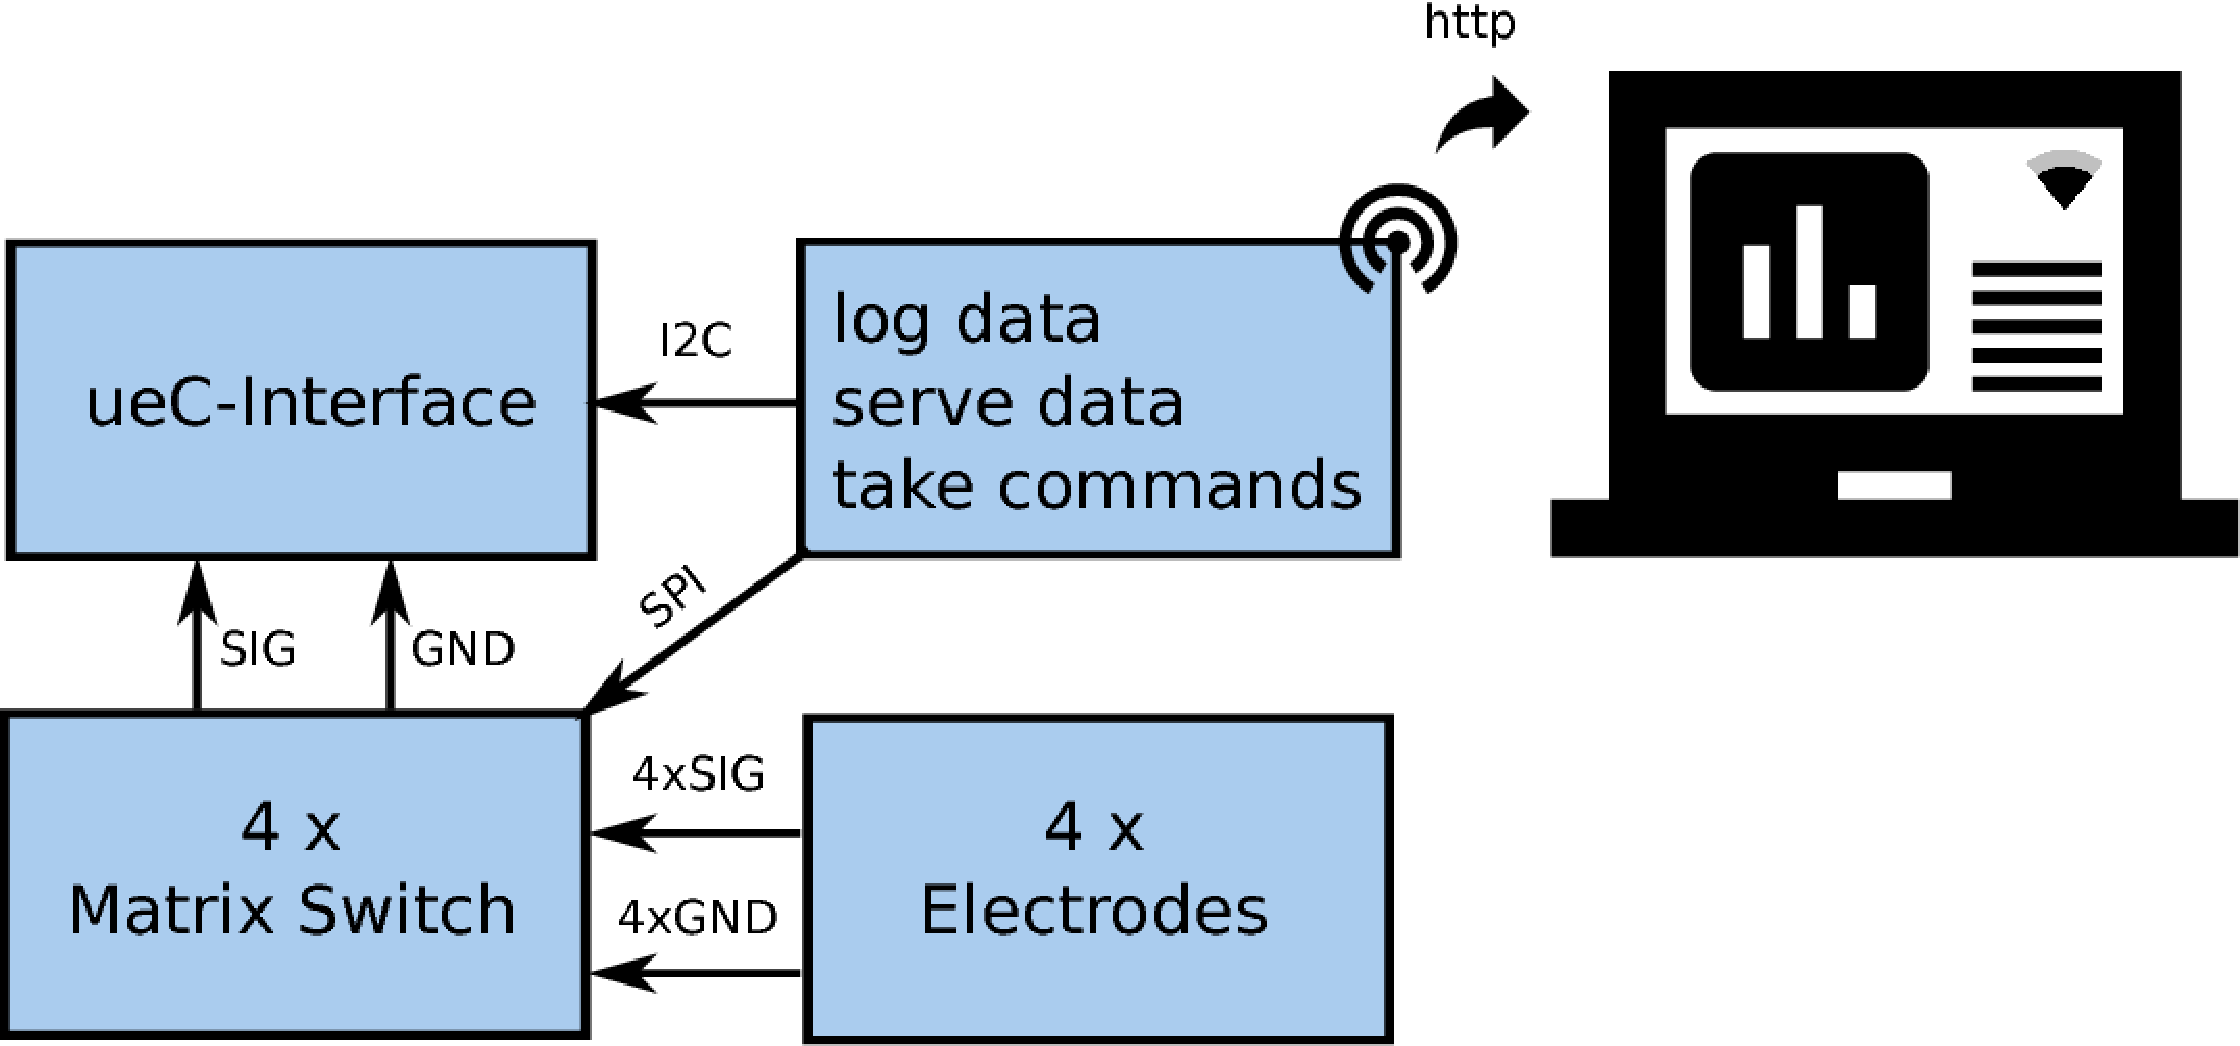
\includegraphics[width=\textwidth]{images/systemdesign.pdf} 
		\caption{System Design}
		\label{fig:sys}
	\end{center}
\end{figure}

\section{Electrodes}

The electrode pairs are the actual sensors in contact with the fluid to be measured. Their material and geometry influence the measuring range of the system. According to information in the book \cite{trankler2015sensortechnik} a cell constant $ C $ of $1$ enables a range from \unitfrac[$2 \cdot 10^3$]{$\mu S$}{cm} to \unitfrac[$10 \cdot 10^3$]{$\mu S$}{cm}. For a water temperature of \unit[$18^\circ$]{C} this corresponds to salinities of \unit[0.66]{\%} and \unit[0.12]{\%}. While this theoretical range is not sufficient for our purpose, first tests showed that the achievable range is much bigger than described in the book. The book doesn't specify the materials influence on the range and it also doesn't qualify how the usable range is defined. As our application has much lower demands on accuracy as the usual ones, this might be an explanation for the discrepancy. \\

Figure \ref{fig:sensor} shows the geometry of the sensor. To achieve a cell constant $C$ of $1$, a width $w$ of \unit[1]{mm}, height $h$ of \unit[10]{mm} and distance $d$ of \unit[10]{mm} were chosen.\\

\begin{figure}[H]
	\begin{center}
		\begin{tikzpicture}
			\draw [line width=0.5mm] (-1,-1) -- (-1,1) -- (-1.3,1) -- (-1.3,-1) -- (-1,-1);
			\draw [dash dot] (-1.15,-1.5) -- (-1.15,1.2);
			\draw [line width=0.5mm] (1,-1) -- (1,1) -- (1.3,1) -- (1.3,-1) -- (1,-1);
			\draw [dash dot] (1.15,-1.5) -- (1.15,1.2);

			\draw (-1,1.6) -- (-1,1);
			\draw (-1.3,1.6) -- (-1.3,1);
			\draw (-1,1.4) -- (-1.3,1.4) node[above, pos=-0.75] {$w$};
			\draw [arrow]  (-1.7,1.4) -- (-1.3,1.4);
			\draw [arrow] (-0.6,1.4) -- (-1,1.4);
			
			\draw (-1.9,1) -- (-1.3,1);
			\draw (-1.9,-1) -- (-1.3,-1);
			\draw [darrow] (-1.7,1) -- (-1.7,-1) node[left, pos=0.5] {$h$};

			\draw [darrow] (-1.15,-1.3) -- (1.15,-1.3) node[above, pos=0.5] {$d$};

		\end{tikzpicture}
		\caption{An electrode pair forming a sensor.}
		\label{fig:sensor}
	\end{center}
\end{figure}

As a first proof-of-concept a sensor array was built, containing multiple electrode pairs on a strip, pictured in figure \ref{fig:v2}. A \unit[5]{cm} wide and \unit[25]{cm} long band of Kapton adhesive tape served as the base. 4 electrode pairs made from \unit[0.2]{mm} platinum wire were arranged equidistant on the strip. \unit[0.4]{mm} enameled copper wire runs along the tape to connect each electrode pair to the left end of the strip, from which insulated cables run to the sensor node. After soldering the joints, two smaller strips of tape were used to cover the wiring, exposing only the electrodes to fluid.

First tests with this sensor array showed the viability of the concept, however a simple look at it shows the inherit problems. Instead of a uniformly flat strip with minimal influence on the flow, the assembly forms several irregularities. Soldering \unit[0.2]{mm} platinum wire to \unit[0.4]{mm} enameled copper wire on a piece of adhesive tape per hand also did not result in clean solder joints. And while with the experience of the first array, the second array turned out a bit cleaner, the fundamental problem remains: it is a tedious manufacturing process resulting in a low quality product.

\begin{figure}
	\begin{center}
		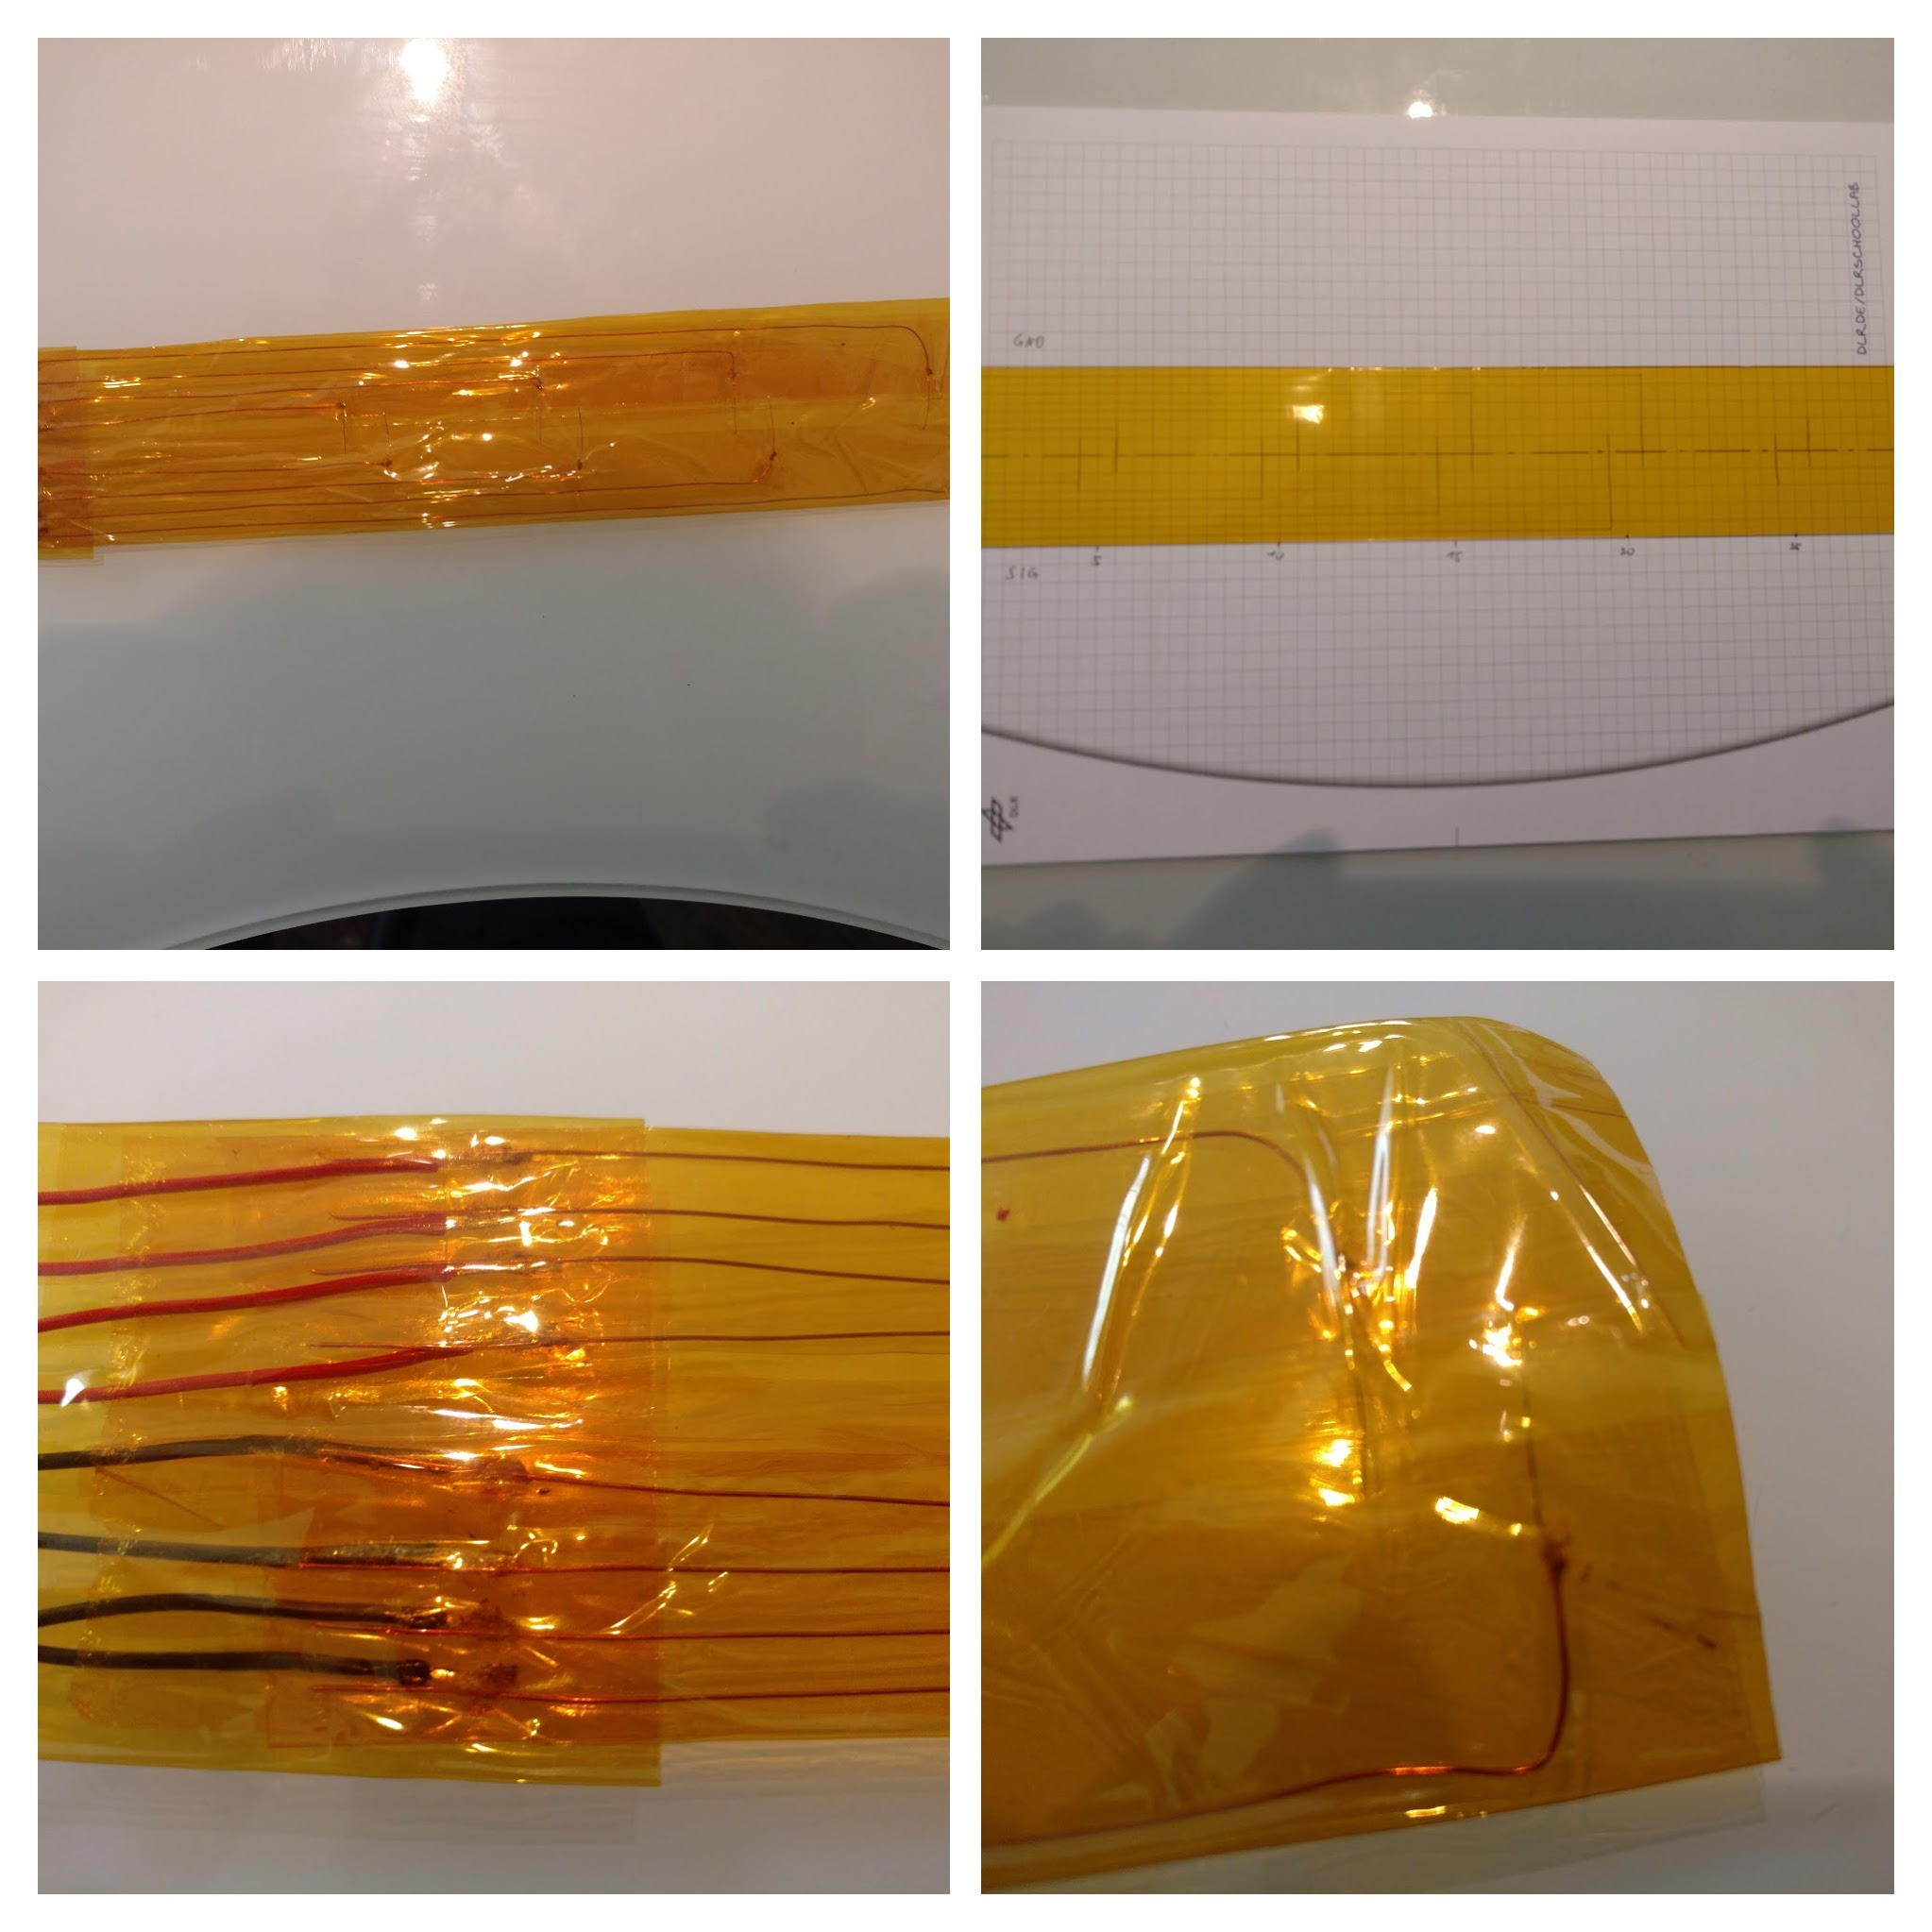
\includegraphics[width=\textwidth]{images/v2.jpg} 
		\caption{A handmade sensor strip.}
		\label{fig:v2}
	\end{center}
\end{figure}

As an alternative to these handmade strips, industrially produced Flex-PCBs were identified. Flex-PCBs are flexible printed circuit boards that are very close to the handmade arrays described above. They also use Kapton as base, on which a copper coating gets applied and partially removed by etching to form the conducting paths. On top, another layer of Kapton is applied, with cutouts in the places where the copper is supposed to be exposed. The exposed copper is then plated with ENIG (Electroless nickel immersion gold) to protect the copper from oxidation and provide the landing pads for electrical components to be soldered on.

For our purpose those exposed and plated landing pads can be used as electrodes, being nicely embedded in a FlexPCB that also runs the wiring up to an interface from where cables can be run. Using the FlexPCB itself as cable is not viable due to the high cost per area. Instead, cables are soldered directly to the PCB and silicone is used to create a waterproof seal around the connection.\\

The final design for the sensor strip, as shown in figure \ref{fig:fpcbd}, implemented as a flexible PCB consisted of 4 electrode pairs spaced \unit[50]{mm} apart. The strip is \unit[25]{mm} wide and \unit[220]{mm} long. 16 pieces were manufactured by LEITON for a price of \euro{376.47}, resulting in a price per strip of \euro{23.53} and of \euro{2.94} per sensor. Figure \ref{fig:fpcbp} shows a sensor strip with attached cables an silicone waterproofing.

\begin{figure}
	\begin{center}
		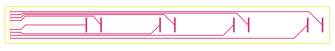
\includegraphics[width=\textwidth]{images/fpcbd.pdf} 
		\caption{The sensor strip design to be implemented as flexible PCB.}
		\label{fig:fpcbd}
	\end{center}
\end{figure}

\begin{figure}
	\begin{center}
		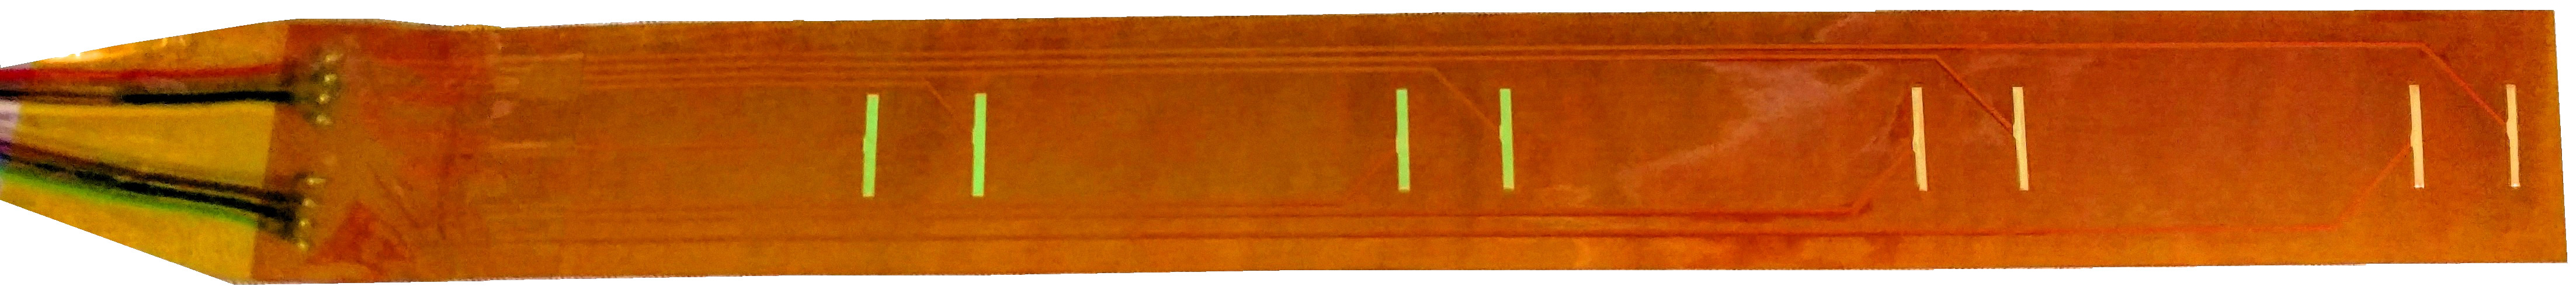
\includegraphics[width=\textwidth]{images/fpcbp.jpg} 
		\caption{A sensor strip manufactured by LEITON and assembled with cables and waterproofing.}
		\label{fig:fpcbp}
	\end{center}
\end{figure}

\section{Matrix Switches}

The matrix switches are an essential part of the system, enabling it use multiple sensors with a single MinieC Interface, thus lowering the cost per sensor. The part used is an ADG738 from Analog Devices. It is an 8-channel CMOS analog matrix switch controlled via a 3-wire serial interface. The following information is taken from the data sheet \cite{ms}.\\

Figure \ref{fig:ms} shows the functional block diagram. The switch has one drain pin (D) and 8 source pins (S1..S8). Despite the naming of drain and source, the internals provide simple switches between the drain and each source pin. The switches work in both directions without any restriction on the signal beyond a maximum current of \unit[120]{mA} that far exceeds our needs. By sending control commands via the 3-wire interface, each of the 8 internal switches can be turned on and off individually.\\

\begin{figure}
	\begin{center}
		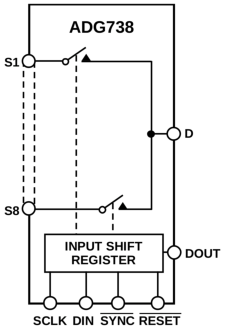
\includegraphics[width=0.3\textwidth]{images/ms.pdf} 
		\caption{Functional block diagram of ADG738}
		\label{fig:ms}
	\end{center}
\end{figure}

The example timing diagram \ref{fig:msc} describes the data transmission process. The microcontroller sends one byte of data to the matrix switch. Each of the 8 bits of this byte controls one switch. The first bit controls the first switch and so on. If the bit is 1, the switch is closed, if 0, the switch is open. To send the byte, first the synchronization pin (SYNC) has to be pulled low from it's usual high level. A clock signal is provided to the clock pin (SCLK). At each falling edge of the clock signal, the data input (DIN) is read - where high leads to a 1-bit and low to a zero-bit. After 8 cycles, SYNC is pulled high again marking the end of data transmission with a full byte transferred. After that, the switches immediately take their instructed states with switching times in the order of \unit[100]{ns}. In the example shown, the first switch is on, while all others are off.\\

\begin{figure}
	\begin{center}
	\tikzexternaldisable
		\begin{tikztimingtable}
  			SYNC   & H 32{L} H \\
  			SCLK   & C 16{2C} N(A1) C \\
  			DIN  	& 2{L} {2H} N(B1) 15{2L} \\
  			Data	& 2D{} 2D{1} 2D{} 2D{0} 2D{} 2D{0} 2D{} 2D{0} 2D{} 2D{0} 2D{} 2D{0} 2D{} 2D{0} 2D{} 2D{0} 2D{}\\
		\end{tikztimingtable}
		\caption{Timing diagram}
		\label{fig:msc}
	\end{center}
\end{figure}

Multiple matrix switches can be controlled at once by daisy-chaining the data output pin (DOUT) of the first device to DIN of the second one, and on so forth. Both SYNC and SCLK are connected to the same bus. This assures that all matrix switches are set in the same state and at the same time.

\section{MinieC Interface}

The MinieC Interface contains the electronics to perform the resistance measurement. It contains sever parts used to generate an electrical signal, run it through a circuit in which the liquid to be measured serves as a resistor and measure the voltage drop over it.\\

The first part is a TPS6040 charge pump voltage inverter. It's purpose is to generate a negative output voltage from a positive input. This negative voltage and the positive voltage are needed to drive a Wien bridge oscillator. This oscillator outputs a sine wave voltage oscillating between the positive and negative input voltage. This whole first stages purpose is to generate an alternating current to be used in the measurement, avoiding the polarization effects described in the background chapter.\\

The AC signal provided by the first stage is then fed into an OpAmp. An OpAmp is a part that has two input signals and one output, where the output is proportional to the difference of the input signals. In our use case, the OpAmp's output is pulled to ground via a voltage divider. The first resistor $R_i$ in the divider is fixed, while the second one $R$ is the liquid to be measured. The output voltage of this divider is depended on the liquids resistance. This voltage is then fed back into the second input of the OpAmp. Via this feedback, the output (OUT) of the OpAmp is now the input signal (SIG) modulated in amplitude by the resistance of the liquid.

\begin{figure}[H]
	\begin{center}
		\begin{circuitikz}
			\draw
				(0,0) node[op amp, yscale=-1](oa1) {}
				(oa1.+) node[left] {SIG}
				(oa1.out) to[R=$R_i$] +(0,-2) coordinate (fb)
			    to[vR=$R$] +(0,-2)
			    to +(0,0) node[ground] {}
			   (fb) to[short, o-] +(-3,2) coordinate (i1)
			   (oa1.-) to[short] +(0,1.5) coordinate (i2)
			   (i1) to (i2)
			   (oa1.out) to[short, o-] +(1,0) coordinate (out)
			   (out) node[right] {OUT}
				;
		\end{circuitikz}
		\caption{OpAmp}
		\label{fig:opamp}
	\end{center}
\end{figure}

In the last step, the modulated output is amplified in two stages, filtered, and then measured by an analog-digital-converter (ADC). The ADC measures the voltage and provides the measurement to the microcontroller via I2C.\\

First test of the interface surfaced an interesting problem. The graph displayed in figure \ref{fig:swcap} shows the response to an immediate switch from the AC input signal to zero. The first red line marks the moment of the switch, the second line marks the moment when the response reached the voltage zero. The red dot marks the moment when the response reached the midpoint between the old and new input. It took \unit[40]{ms} for the response to follow the input. This slow response time is not acceptable in our system because it prohibits the switching between sensors. The slow response would smear the measurement over all sensors and it would not be possible to measure a difference between them. Waiting for that amount of time between each read of a sensor would reduce the time resolution to a level where the desired information can no longer be extracted from the data. The cause of this behavior is the filter placed before the ADC. As the output of the OpAmp is an alternating current, a diode and a filter capacitor are used to generate a direct current signal proportional to the amplitude of the AC signal. This is done so the sample rate of the ADC does not have to match the frequency of the signal, which makes it easier to use when fast sampling rates are not necessary.\\

\begin{figure}
	\begin{center}
		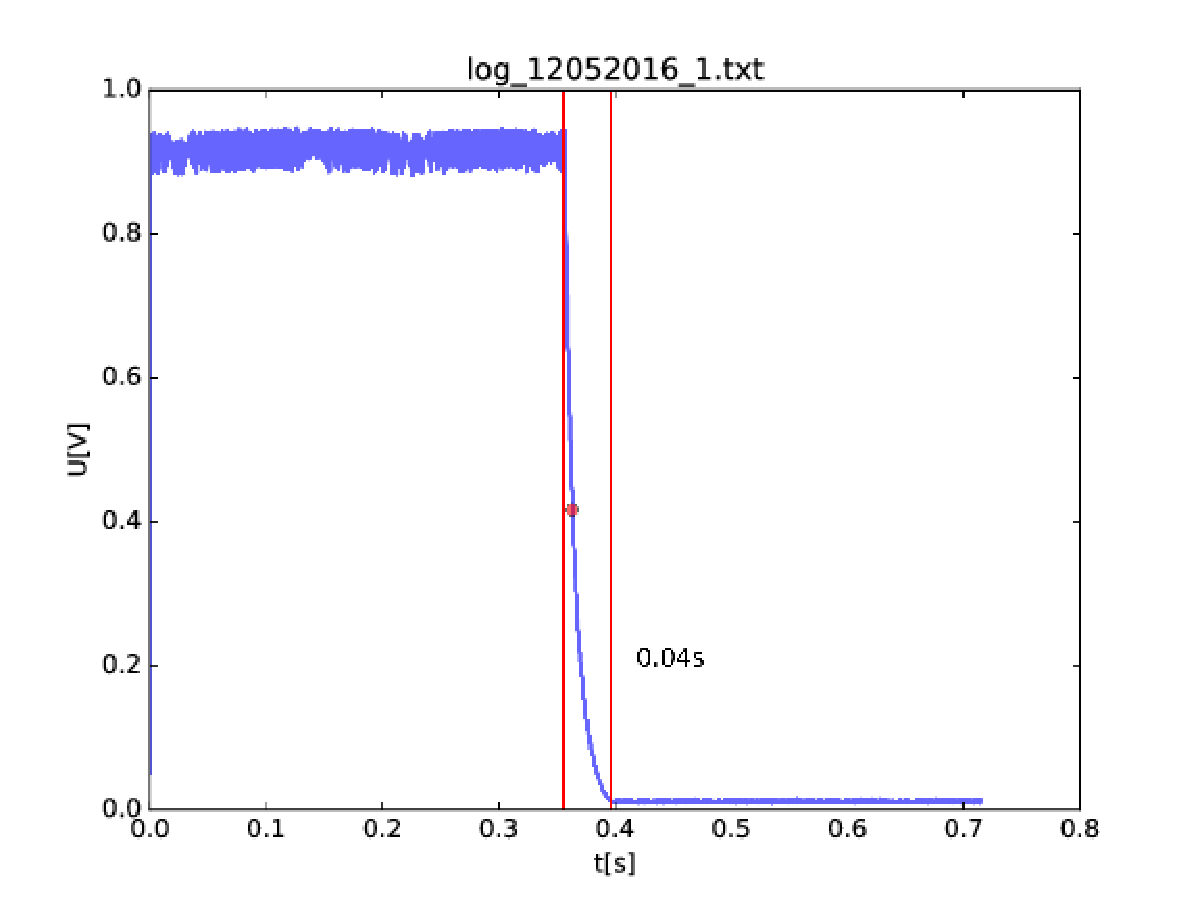
\includegraphics[width=0.8\textwidth]{images/switch_cap.pdf} 
		\caption{After the switch, the capacitor discharges slowly.}
		\label{fig:swcap}
	\end{center}
\end{figure}

Figure \ref{fig:swnocap} shows the response to the same switching as before, but with the filter capacitor removed. The diode is still in place and removes the negative voltages from the output. Without the capacitor however, the signal oscillates with the same \unit[1666]{Hz} as the Wien bridge oscillator provides. Because the sample rate of the ADC is not as fast as the oscillation, it measures at random moments on the sine wave, resulting in an output that moves between zero and the maximum amplitude. The red line again marks the moment of the switch and it can be clearly seen that the response delay is now gone. The oscillating behavior that was electrically filtered before, now can be filtered digitally without the sensors influencing each other.

\begin{figure}
	\begin{center}
		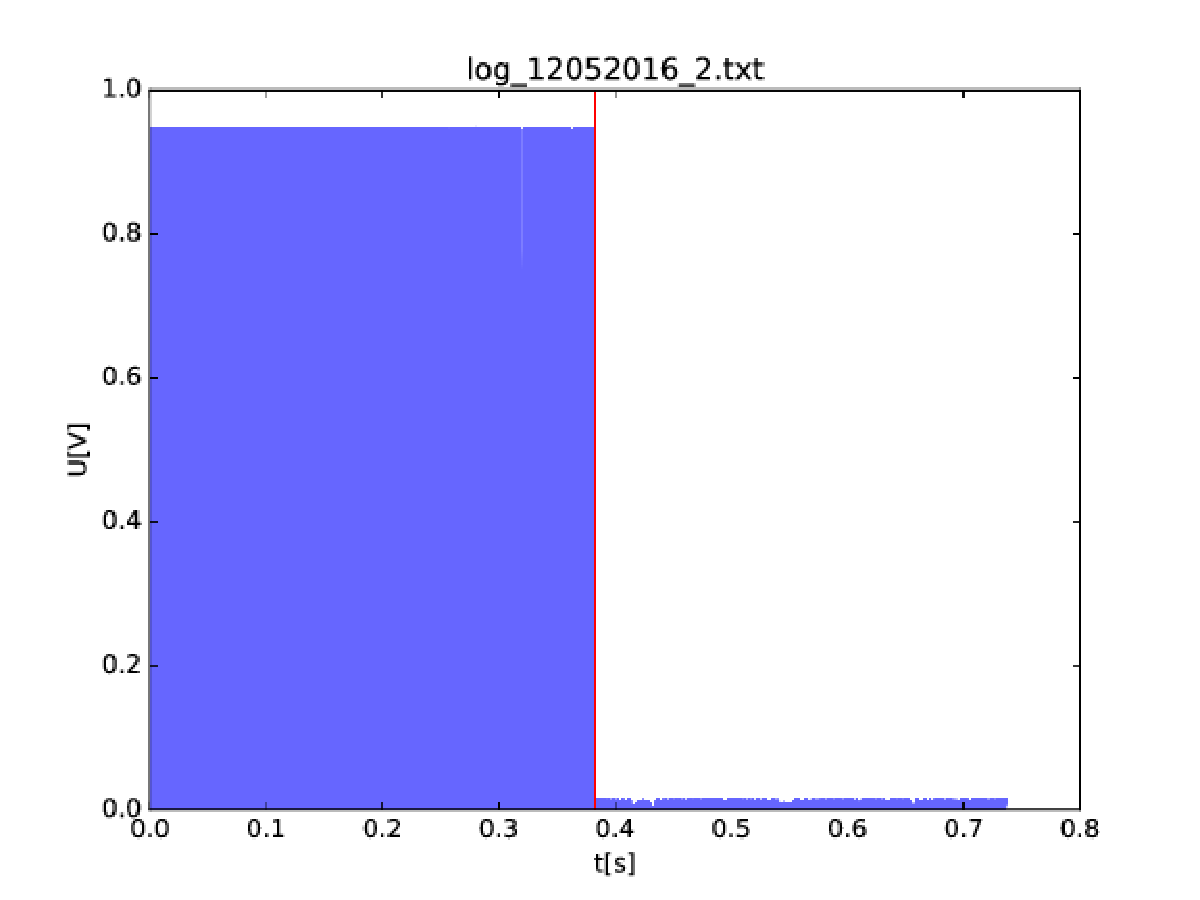
\includegraphics[width=0.8\textwidth]{images/switch_nocap.pdf} 
		\caption{The response immediately follows the switching event, but the AC signal is now unfiltered.}
		\label{fig:swnocap}
	\end{center}
\end{figure}

\section{Microcontroller} \label{uc}

The microcontroller has to be able to control the functions of the sensor nodes attached to it, read the data from them, log it and serve it to the user-interface. They usually are programmed in C or C++, however in recent years other options emerged. One of those is Micropython, which is an implementation of the Python 3 programming language designed to run on microcontrollers. Python is a vastly easier language to work with than C/C++, and this is especially true when the involved persons are not from a computer science or electrical engineering background, but i.e. mechanical engineering or other sciences. In those fields, Python is often familiar from usage for data processing and visualization. Using Micropython enables us to design a system where it is more likely that the people using it are able to understand the code, enabling them to improve it and adapt it to alternate use-cases.
It does however limit our choice of hardware to supported platforms and it requires more powerful and thereby expensive micro-controllers. But as the system only requires one microcontroller to drive a very large amount of sensors, the added cost is relative and outweighed by the benefits of the better usability.\\

For prototyping, a development board named "Espruino Pico" was chosen. It is a very small and simple board that provides the electrical boilerplate to use a micro-controller without needing to deal with the lowest level of electronics, like cleaning power supply, USB connection and so on. The board costs \euro{35}.\\

\section{Carrier Board}

The carrier board is a simple PCB implementing all parts described above. Figure \ref{fig:cb} shows the assembled board. On the left, the Espruino Pico board can either be soldered directly to the PCB or plugged in using pin header connectors. Above and beyond used pins are replicated on through-holes. This allows for easy connection of measurement equipment to debug the system during development, but can also be used later to connect carrier boards together. Only one would carry a microcontroller and control the other connected boards.

In the middle there are two matrix switches. They can either be directly soldered on as in this image or they can be soldered to an adapter board that is again mounted to the carrier with pin header connectors in the inner rows of through-holes.  The outer through-holes are where the connectors for the cables to the sensors are mounted.

On the right side the MineeC Interface is mounted. It also can be either directly soldered or use pin header connectors.

The design is tailored to the use as a prototype. That means that everything is made a bit bigger than necessary, which allows for easier modifications. It also is kept modular, so that each part can be swapped out easily. A later redesign would integrate all boards into one and try to reduce size, which in turn saves money on PCB manufacturing. However, the prototype showed no design errors and is fully functional, so the next design step is only necessary when more boards are needed.

The carrier boards were manufactured by dirtypcbs, a very cheap service for prototype boards. The total cost for 10 pieces was around \euro{50}, depending on conversion rates, of which about \euro{30} were shipping costs from China to Germany. The low price comes with low quality, as the name of the service already suggests, but for prototypes the trade-off is well worth it.

\begin{figure}
	\begin{center}
		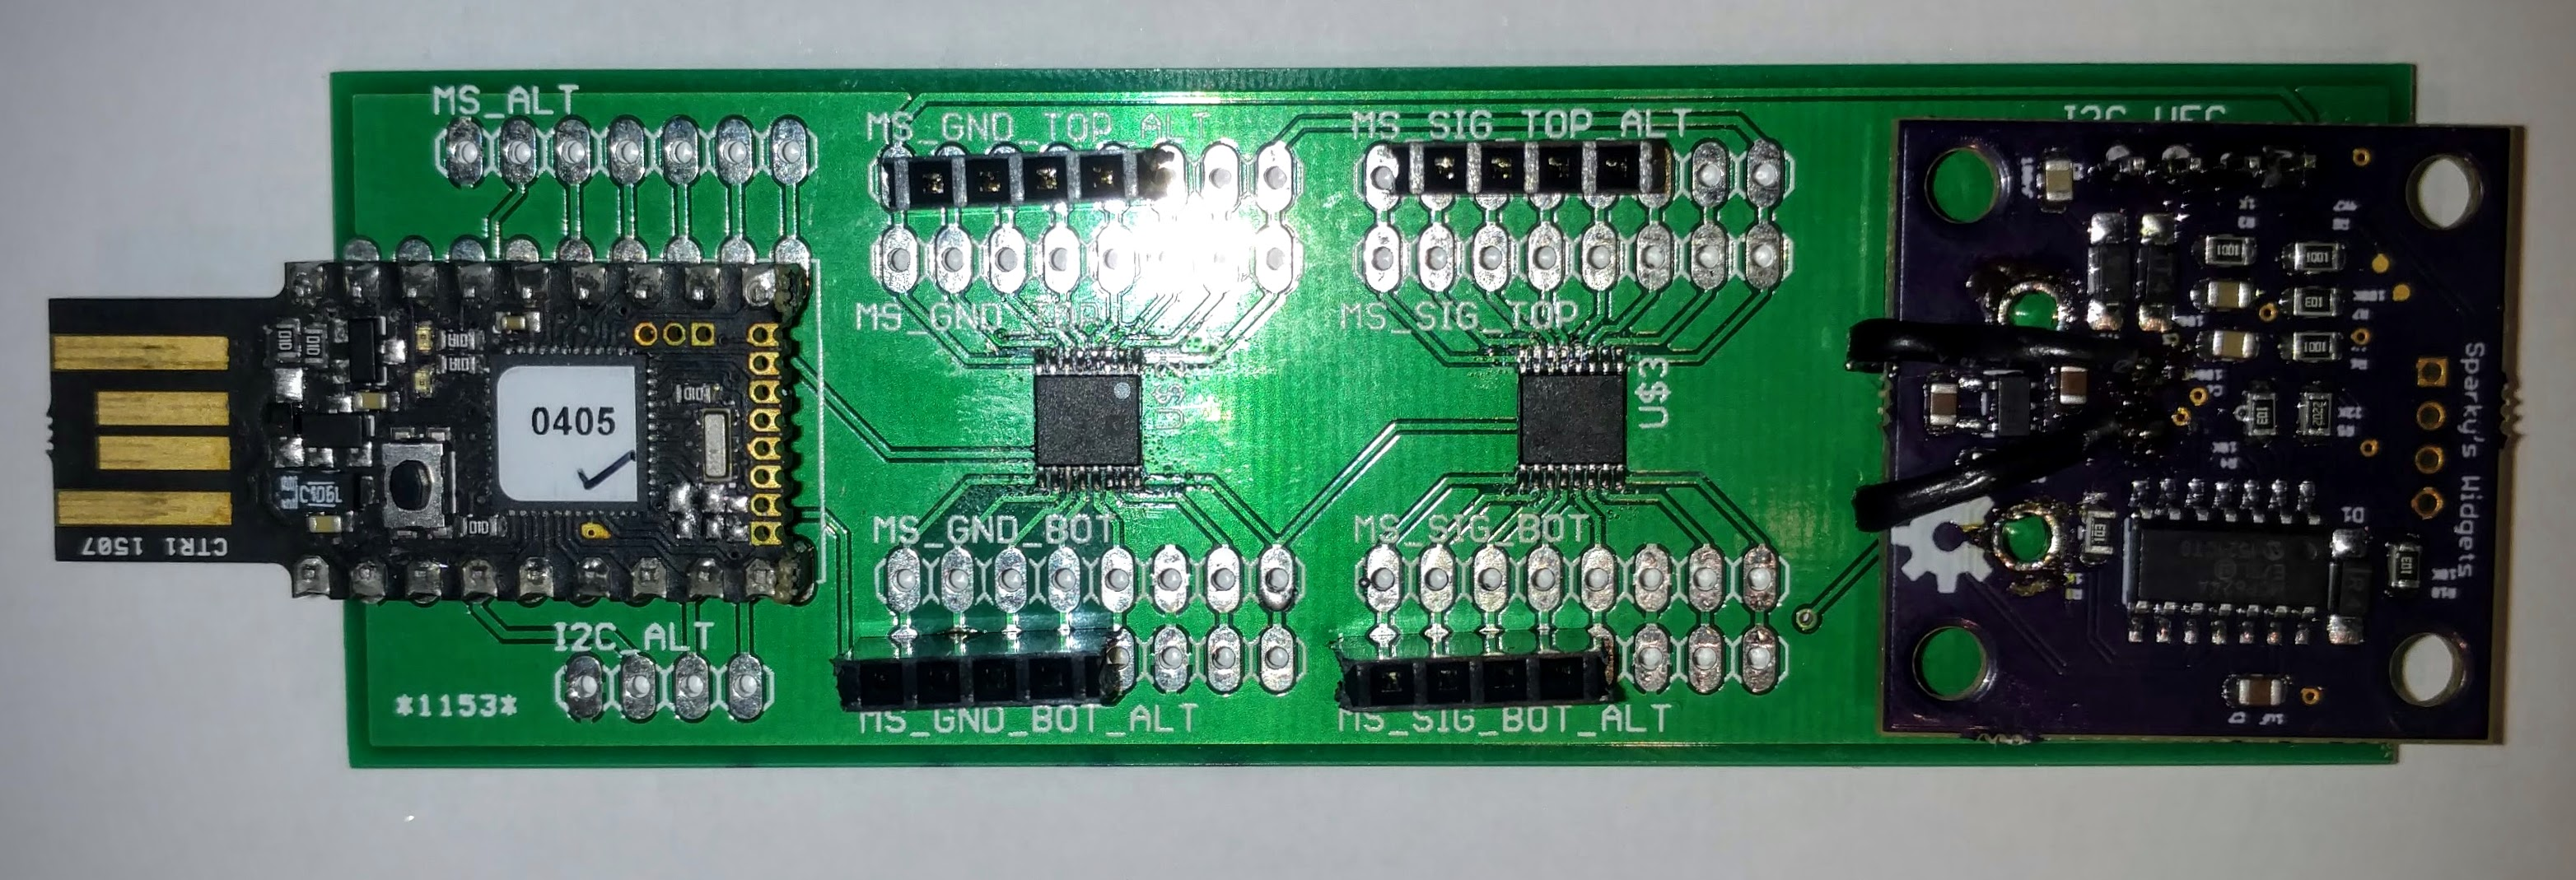
\includegraphics[width=0.8\textwidth]{images/cb.jpg} 
		\caption{The assembled carrier boar with all parts mounted.}
		\label{fig:cb}
	\end{center}
\end{figure}

\section{Embedded Software}

The embedded software is the program running on the microcontroller. As already described in section \ref{uc}, Micropython is used to implement this program.\\

As soon as the system is powered up, it starts listening for the Start and Stop commands from the OpenSalinity GUI running on the host PC. Once it receives the Start command, it starts polling the sensors and delivers the data to PC, where it is captured.
In order to poll the sensors, the program has to control the switches and the ADC. It first switches both matrix switches to a certain electrode pair and then reads the ADC value for it. After that it switches to next pair and thus circles through all connected sensors. Each ADC read is accompanied by a time stamp for the read.\\

The data is sent in a simple format described in the listing \ref{format}. One line contains timestamps and values for all $n$ connected sensors separated by one whitespace. The line ends with the newline character.

\begin{figure}[H]
\begin{center}
\begin{lstlisting}
<time 1> <value 1> <time 2> <value 2> ... <time n> <value n> \n
\end{lstlisting}
\caption{Data Format}
\label{format}
\end{center}
\end{figure}

\begin{figure}
	\begin{center}
\begin{tikzpicture}[scale=1]
	%\begin{pgfonlayer}{nodelayer}
		\node [style=scircle, inner sep=8pt] (0) at (0, 15) {power on};
		\node [style=diamond, inner sep=8pt, align=center] (1) at (0, 10) {read\\command\\from GUI};
		\node [style=rect, inner sep=8pt, align=center] (2) at (0, 6) {switch to\\sensor n};
		\node [style=rect, inner sep=8pt, align=center] (3) at (0, 4) {read ADC};
		\node [style=rect, inner sep=8pt, align=center] (4) at (0, 2) {create\\timestamp};
		\node [style=rect, inner sep=8pt, align=center] (5) at (0, 0) {send data\\to GUI};
	%\end{pgfonlayer}
	%\begin{pgfonlayer}{edgelayer}
		\draw [style=arrow] (0) to (1);
		\draw [style=arrow] (1) to node[right, pos=0.1]{Start} (2);
		\draw [style=arrow] (2) to (3);
		\draw [style=arrow] (3) to (4);
		\draw [style=arrow, bend right=90, looseness=1.00, align=left] (4) to node[right]{n++\\while n < sensors} (2);
		%\draw [style=simple, in=90, out=0, loop] (1) to node[above, pos=0.01]{Stop} (1);
		\draw [style=simple, in=90, out=0, looseness=2.5] (1.east) to node[below, pos=0.1, yshift=-4pt]{Stop} (1.north);
		\draw [style=arrow] (4) to (5);
		\draw [style=arrow, in=-180, out=-90, looseness=1.25] (5) to (1);
	%\end{pgfonlayer}
\end{tikzpicture}
		\caption{Embedded Software Flow Diagram}
		\label{fig:flow}
	\end{center}
\end{figure}

\section{OpenSalinity GUI}

The OpenSalinity GUI is a program designed to simplify and aid the usage of the sensor system. It provides following functionality:

\begin{itemize}
	\item Storing all sensor data to a file.
	\item Choosing a file to which the data is stored.
	\item Starting and Stopping the data capture.
	\item Visualize the data.
\end{itemize}

The data capturing can not be started before a file to save to is chosen, to avoid the unintentional loss of data. The Save button allows to create the file to be written to and offers a default file name containing the date and time of the creation, helping to keep the data logs in order.
The live visualization is a bar graph showing each sensors current measurement, allowing to monitor the ongoing experiment. In addition to size, the bars are also color coded, shifting from red to blue with increasing salinity.\\

\begin{figure}[H]
	\begin{center}
		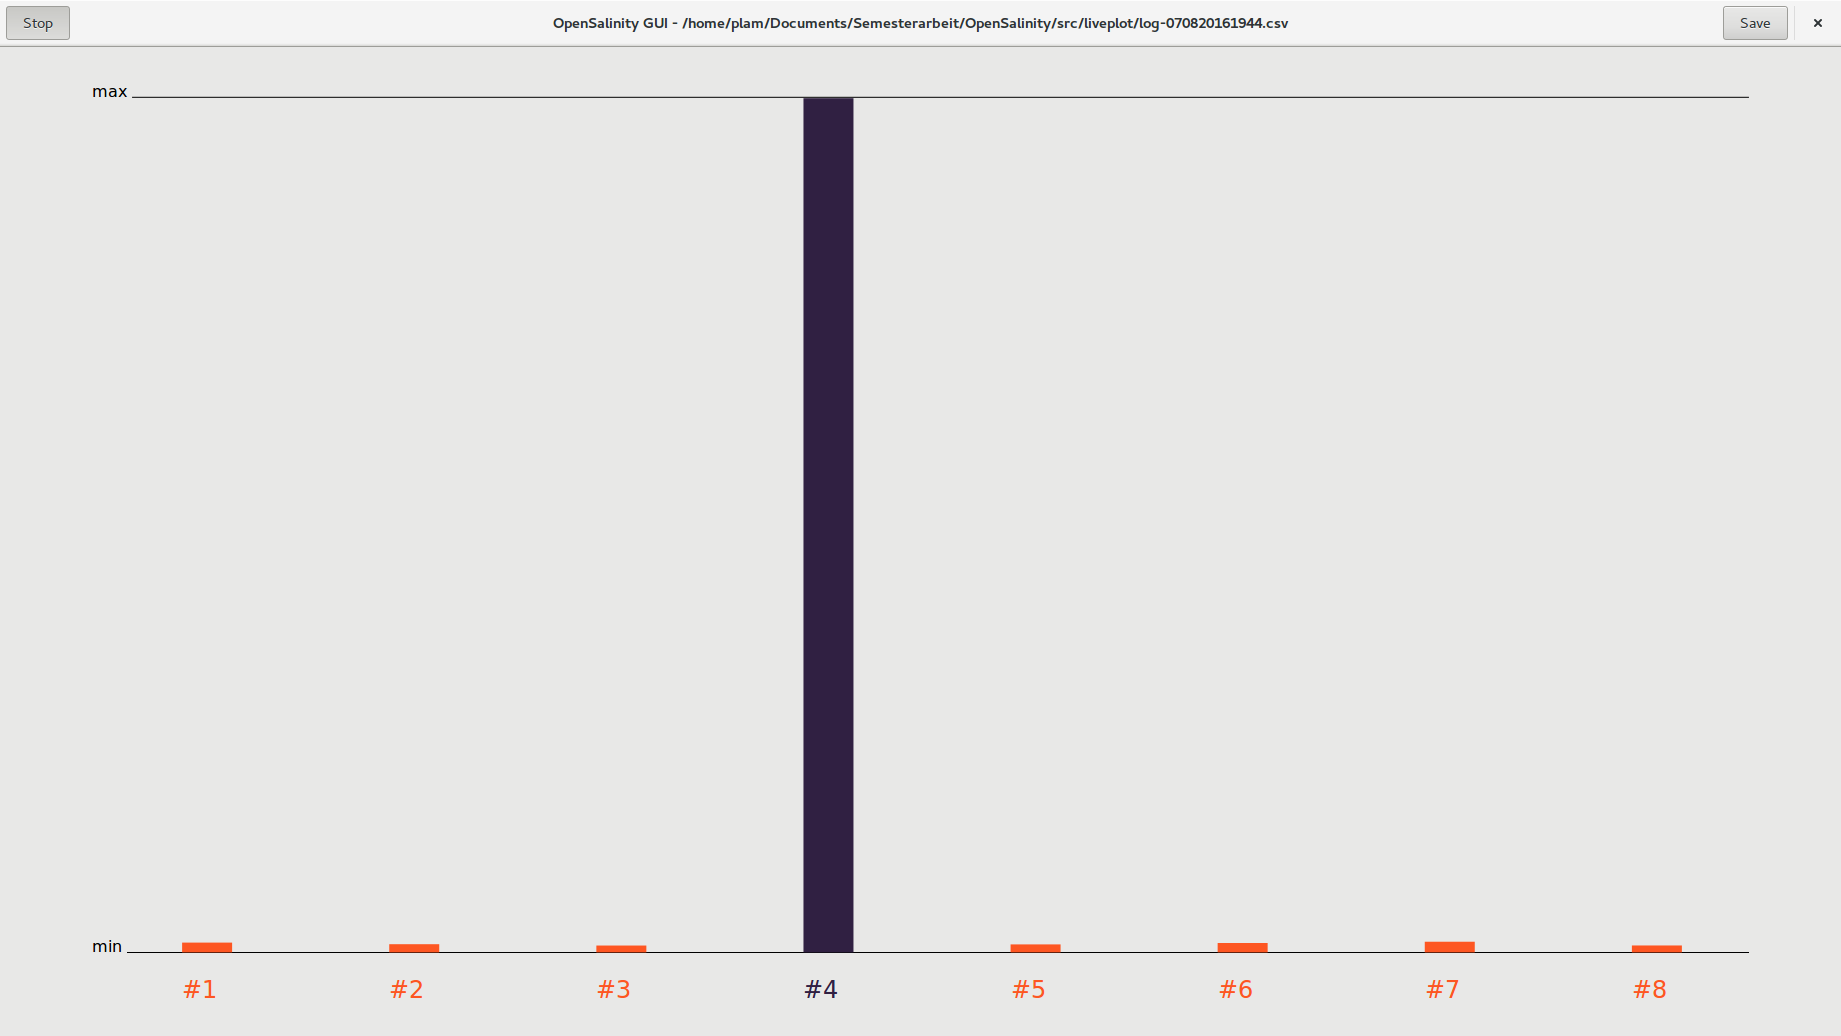
\includegraphics[width=\textwidth]{images/UI.png}
		\caption{OpenSalinity GUI}
		\label{fig:opamp}
	\end{center}
\end{figure}

The software again is written in Python, using GTK+ as GUI toolkit and pyserial to communicate with the microcontroller. It was developed and testes on a Linux based operating system, however due the nature of the used programming language and toolkits it is cross-platform and can be run on Windows and OSX also.\\

In addition to or as replacement of the GUI, a set of command line tools can be used. These tools allow for a redundant capturing of the sensor data and for an alternate visualization. A detailed manual on how to use those tools as wells as the GUI is provided in the Appendix.

\section{Data Conditioning}

Before the data can be analyzed it has to be conditioned to deal with certain quirks of the embedded software. This is done in post processing rather than live to minimize overhead on the microcontroller to retain high sampling rates.\\

The data conditioning scans through the data and generates a rolling time from the wrapping times. The microcontroller measures time since start up by counting clock cycles. These are converted to microseconds stored as an integer value. The microcontroller is a 32-bit architecture, however the Micropython implementation uses 2 bits for data type identification, leaving 30 bits for data. This means the counter can count from $-2147483647$ to $2147483647$, meaning that it wraps around roughly every $8.9$ minutes.\\